\chapter{Transporte Óptimo de Masas}
En este capítulo se abordará el problema de transporte óptimo, la distancia de Wasserstein, y el problema de los baricentros de Wasserstein. Además, se presentarán algunas propiedades de la distancia de Wasserstein, las cuales serán de utilidad en el desarrollo de este trabajo. La notación y definiciones utilizadas en este capítulo se encuentran basadas en \cite{villani2009optimal} y \cite{peyre2019computational}. Sin embargo, antes de empezar a enunciar definiciones y propiedades, se sentarán la notación y definiciones básicas que se utilizarán a lo largo de este trabajo.
\JF{Un comentario}

\section{Notación}
 {
  \FM[inline]{Agregar alguna intro para lo que es una medida de probabilidad? para aquellas personas que vienen de otras áreas?}
  \begin{definition}
	  \FM[inline]{Se podría dejar notación probabilística?}
	  Se definen los siguientes espacios:
	  \begin{itemize}
		  \item $(\cX, \dist)$ es un espacio Polaco, si $\cX$ es un espacio métrico, completo y separable.
		  \item $\ProbSpace[\cX]$ denotará al conjunto de medidas de probabilidad en $\cX$, utilizando la $\sigma$-álgebra de Borel.
		  \item $\ProbSpaceAC[\cX]$ denotará al conjunto de medidas de probabilidad absolutamente continuas con respecto a una medida de referencia $\lambda$ (como por ejemplo, la de Lebesgue o la cuenta puntos), utilizando la $\sigma$-álgebra de Borel.
		  \item $\mathcal{C}(\cX)$ denotará al conjunto de funciones continuas en $\cX$.
		  \item ${\Lip}_{k}(\cX)$ denotará al conjunto de funciones $k$-Lipschitz en $\cX$. Mientras que se asumirá que $\Lip[\cX]$ denotará al conjunto de funciones $1$-Lipschitz en $\cX$. \FM[inline]{Se podría agregar una definición de función Lipschitz?}
	  \end{itemize}
  \end{definition}

  \begin{definition}
	  Se definirá el \emph{simplex} de dimension $n$ como el conjunto de vectores de $\R^{n}$ cuyas componentes suman 1, es decir,
	  \begin{equation}
		  \Simplex \eqdef \left\{
		  x \in [0, 1]^{n} \colon \sum_{i=1}^{n} x_{i} = 1
		  \right\},
	  \end{equation}
	  y a los elementos pertenecientes al simplex se les llamará \emph{vectores de probabilidad}.
  \end{definition}

  \begin{definition}
	  Dados $\mu \in \ProbSpace[\cX]$ y $\nu \in \ProbSpace[\cY]$, se denotará por $\Cpl(\mu, \nu)$ al conjunto de medidas de probabilidad en $\cX \times \cY$ cuyas proyecciones marginales sean $\mu$ y $\nu$, es decir,
	  \begin{equation}
		  \Cpl(\mu, \nu) \eqdef \left\{
		  \gamma \in \ProbSpace[\cX \times \cY] \colon \gamma(A \times \cY) = \mu(A), \gamma(\cX \times B) = \nu(B), \forall A \subseteq \cX, B \subseteq \cY
		  \right\}.
	  \end{equation}
  \end{definition}

  \begin{definition}
	  Para una función medible $T:\cX \to \cY$ se define el \emph{operador push-forward} de $T$ como la aplicación $\Tpf:\ProbSpace[\cX] \to \ProbSpace[\cY]$ que satisface la siguiente relación:
	  \begin{equation}
		  %   \label{eq:pushForward}
		  \int_{\cX} f(x) \dd{\Tpf\mu(x)} = \int_{\cY} f(T(x)) \dmu[x], \quad \forall f \in \mathcal{C}(\cY),
	  \end{equation}
	  para toda $\mu \in \ProbSpace[\cX]$. Adicionalmente, el operador push-forward se puede definir como aquel operador que satisface la siguiente relación:
	  \begin{equation}
		  \label{eq:pushForward2}
		  \forall A \subseteq \cY \text{ medible}, \quad \Tpf\mu(A) = \mu(T^{-1}(A)).
	  \end{equation}
  \end{definition}

  \begin{remark}
	  Se puede notar que $\Tpf$ preserva la positividad y la masa total, es decir, si $\mu \in \ProbSpace[\cX]$, entonces $\Tpf\mu \in \ProbSpace[\cY]$.
  \end{remark}

  \begin{remark}
	  Para el caso en que la medida $\mu \in \ProbSpace$ sea una medida discreta\footnote{i.e. $\mu = \sum_{i=0}^{n} m_i \delta_{x_i}$ con $m\in\Simplex$, $x_1,\ldots, x_n\in\cX$ y $\delta_x$ la medida de Dirac en $x$}, entonces el operador $\Tpf$ lo que hará será intercambiar la masa de cada punto de $\cX$ a su imagen en $\cY$, es decir,
	  \begin{equation}
		  \label{eq:pushForwardDiscreto}
		  \Tpf\mu = \sum_{i=0}^{n} m_i \delta_{T(x_i)}.
	  \end{equation}

  \end{remark}



 }

\section{El Problema de Transporte}
 {



  \subsection*{El problema de Monge}
  {
	  En esta sección, se tomará la introducción realizada en el libro \emph{An Invitation to Statistics in Wasserstein Space}, de V. Panaretos y Y. Zemel \citeyear{panaretos2020invitation}. En 1781, Monge \cite{monge1781memoire} se hizo la siguiente pregunta: dada una pila de arena y un pozo de igual volumen, ¿Cuál es la forma óptima de transportar la arena al pozo?

	  Utilizando términos matemáticos, el problema se puede formular de la siguiente manera: dado un espacio de arena $\cX$, un espacio de pozo $\cY$ y una función de costo $c: \cX \times \cY \to \R$ que encapsula el esfuerzo de transportar una unidad de arena en el punto $x \in \cX$ a una posición $y \in \cY $ en el pozo. La distribución de la arena es representada por una medida $\mu \in \ProbSpace[\cX]$, y la forma del pozo es descrito por una medida $\nu \in \ProbSpace[\cY] $. Una representación gráfica de la montaña de arena y el pozo se puede apreciar en la Figura~\ref{fig:montanas-arena-pozo}.

	  \begin{figure}[ht]
		  \centering
		  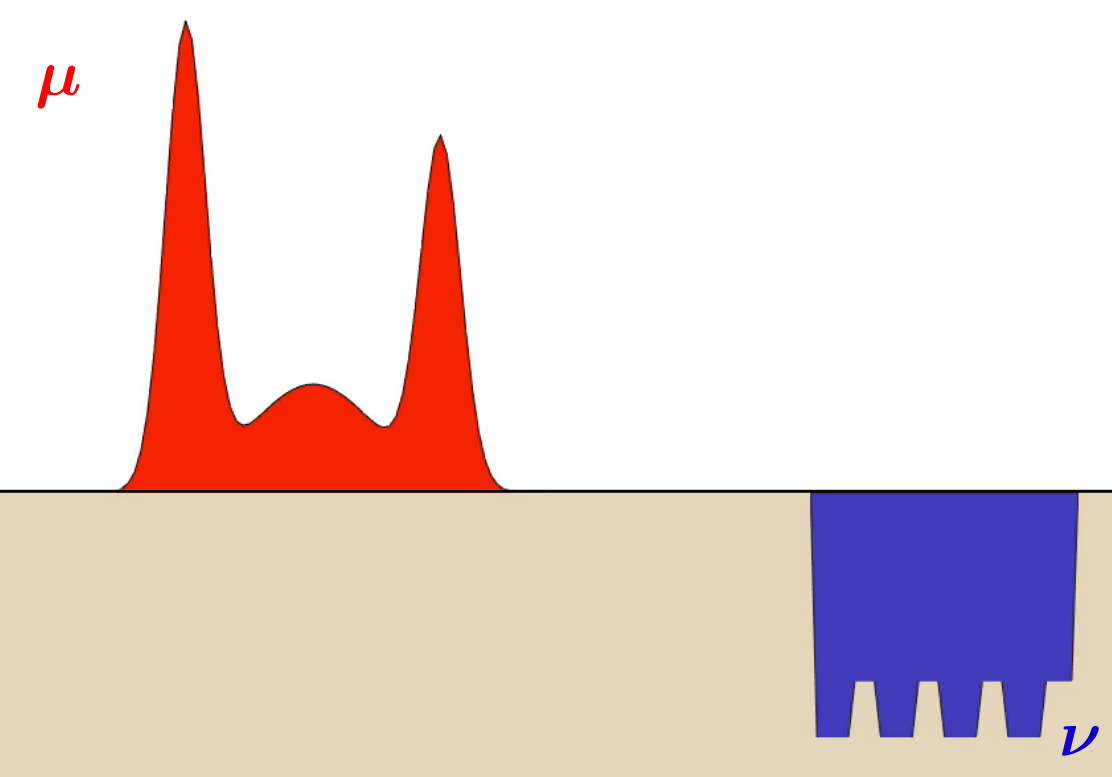
\includegraphics[width=0.5\textwidth]{img/transporte/montanas-arena-pozo.png}
		  \caption{Representación de la montaña de arena, representada en rojo por la medida $\mu$, y el pozo, representada en azul por la medida $\nu$. Imagen obtenida de \cite{cuturi2017primer}.}
		  \label{fig:montanas-arena-pozo}
	  \end{figure}

	  La decisión de cómo transportar la arena es representada por una función $T: \cX \to \cY$, que asigna a cada punto $x \in \cX$ una posición $T(x) \in \cY$ en el pozo. El costo total de transportar la arena al pozo es representado por la siguiente expresión:
	  \begin{equation}\label{eq:costoTotalTransporteMonge}
		  C(T) \eqdef \int_{\cX} c(x, T(x)) \dmu[x].
	  \end{equation}

	  Se puede observar que una propiedad que ha de cumplir la función $T$ es que debe de preservar la masa total de la arena: para cualquier conjunto $B \subseteq \cY$ representando una región en el pozo de volumen $\nu(b)$, debe de ser exactamente el mismo volumen de arena que debe de ir a $B$. La cantidad de arena que está situada en $B$ es $\left\{ x \in \cX : T(x) \in B \right\} = T^{-1}(B)$, y por tanto, la condición de preservación de masa requiere que se cumpla que $\mu(T^{-1}(B)) = \nu(B)$ para toda $B \subseteq \cY$. Esta condición se puede observar gráficamente en la Figura~\ref{fig:preservacion-masa}, y se formula más formalmente a través de la siguiente definición:

	  \begin{definition}[Operador push-forward]
		  Sea una función medible $T:\cX \to \cY$, se define el \emph{operador push-forward}  de $T$ como la aplicación $\Tpf:\ProbSpace[\cX] \to \ProbSpace[\cY]$ que satisface la siguiente relación:
		  \begin{equation}
			  \label{eq:pushForward}
			  \Tpf \mu(B) \eqdef \mu (T^{-1}(B)) = \nu(B),\quad \forall B \subseteq \cY \text{ medible}.
		  \end{equation}
	  \end{definition}

	  \begin{figure}[ht]
		  \centering
		  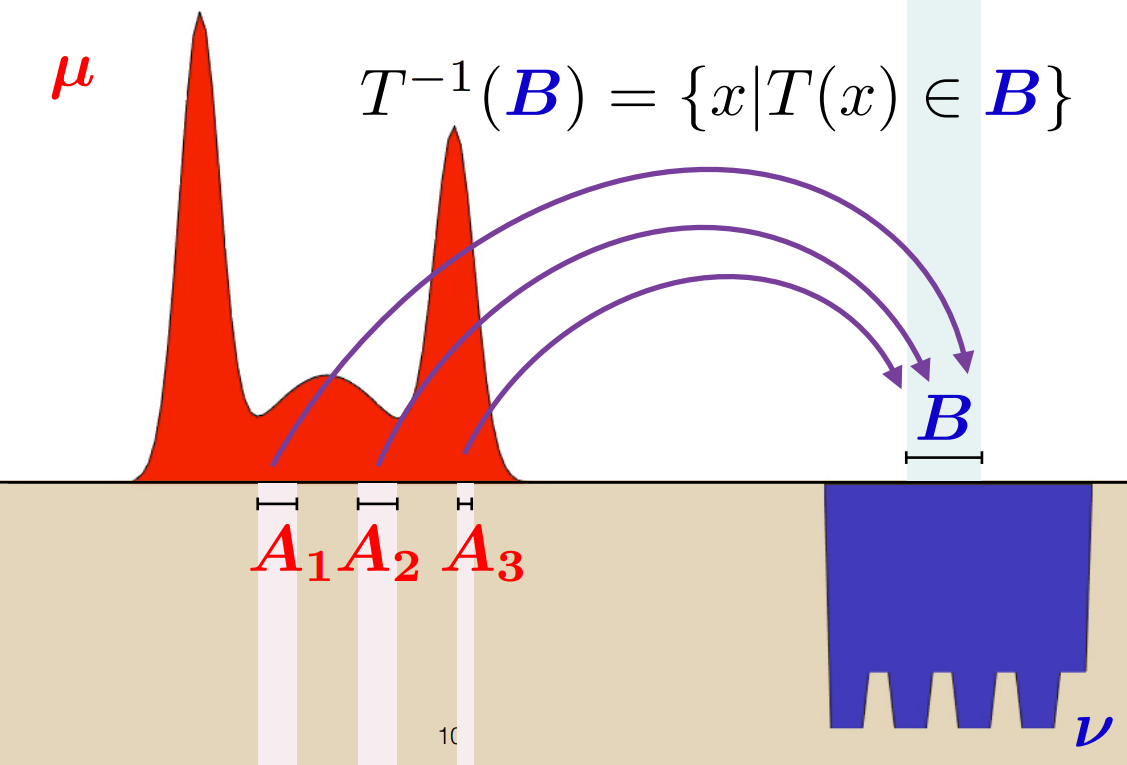
\includegraphics[width=0.5\textwidth]{img/transporte/preservacion-masa.png}
		  \caption{Representación de como la función $T$ ha de preservar la masa total de la arena. Imagen obtenida de \cite{cuturi2017primer}.}
		  \label{fig:preservacion-masa}
	  \end{figure}

	  En este contexto, el problema de Monge consiste en encontrar una función $T: \cX \to \cY$, que minimice el costo total de transporte. Formalmente, este problema se define de la siguiente manera:

	  \begin{definition}[Problema de Monge, \cite{monge1781memoire}]
		  Dadas dos medidas $\mu \in \ProbSpace[\cX]$ y $\nu \in \ProbSpace[\cY]$ y una función de coste $c : \cX \times \cY \to \R$, se define el \emph{problema de transporte óptimo de Monge} como el problema de encontrar una función medible $T: \cX \to \cY$ que minimice el costo total de transporte $C(T)$. Es decir, que minimice la siguiente expresión:
		  \begin{equation}
			  \label{eq:problemaTransporteMonge}
			  \inf_{T: \Tpf \mu = \nu} \int_{\cX} c(x, T(x)) \dmu[x].
		  \end{equation}
		  Aquella función $T$ que resuelva este problema se le llamará \emph{función de transporte} o \emph{mapa de transporte}, y se denotará por $T_{\mu \to \nu}$.
	  \end{definition}

	  El problema introducido por Monge \cite{monge1781memoire} es un problema muy difícil, principalmente porque el conjunto de mapas de transporte $\left\{ T : \Tpf \mu = \nu \right\}$ es intratable. Además, puede que no exista solución alguna, o en caso de haberla, puede que este no sea única, como veremos en los siguientes ejemplos:

	  \begin{example}\label{ex:problemaDeMongeSinSolucion}
		  Consideremos $\cX = \left\{ -1, 1 \right\}$, $\cY = \left\{ 0 \right\}$, con $\mu = \frac{1}{2} \delta_{-1} + \frac{1}{2} \delta_{1}$ y $\nu = \delta_0$. En este caso, la función de transporte óptima que minimiza \eqref{eq:problemaTransporteMonge} es
		  \begin{align*}
			  T_{\mu \to \nu}(-1) & = 0 & T_{\mu \to \nu}(1) & = 0.
		  \end{align*}
		  Sin embargo, se puede notar que no existe transporte óptimo $T_{\nu \to \mu}$  que transporte la masa de $\nu$ a $\mu$, dado que la masa de $\nu$ está concentrada en un único punto, mientras que la masa de $\mu$ está distribuida en dos puntos, y no se puede ``dividir'' la masa. Este correspondería a un ejemplo en el que el problema de Monge no tiene solución.
	  \end{example}

	  \begin{example}\label{ex:problemaDeMongeMultipleSolucion}
		  Consideremos ahora $\cX = \left\{ (1, 1), (-1, -1) \right\}$, $\cY = \left\{ (-1, 1), (1, -1) \right\}$, con $\mu = \frac{1}{2} \delta_{(1, 1)} + \frac{1}{2} \delta_{(-1, -1)}$ y $\nu = \frac{1}{2} \delta_{(-1, 1)} + \frac{1}{2} \delta_{(1, -1)}$. Este ejemplo correspondería a uno en que los puntos de $\cX$ y $\cY$ forman un cuadrado. En este caso, se puede notar que existen dos funciones de transporte óptimo que minimizan \eqref{eq:problemaTransporteMonge}, las cuales son
		  \begin{align*}
			  T^1_{\mu\to\nu}(1, 1) & = (1, -1) & T^1_{\mu\to\nu}(-1, -1) & = (-1, 1)  \\
			  T^2_{\mu\to\nu}(1, 1) & = (-1, 1) & T^2_{\mu\to\nu}(-1, -1) & = (1, -1),
		  \end{align*}
		  comprobando que en este caso, el problema de Monge tiene más de una solución.
	  \end{example}



	  %   \begin{remark}
	  % 	  \label{remark:problemaTransporteMongeDiscreto}
	  % 	  Cuando las medidas $\mu$ y $\nu$ son discretas, es decir, se representan de la siguiente manera:
	  % 	  \begin{align}
	  % 		  \mu & = \sum_{i=1}^{n} a_i \delta_{x_i}, &
	  % 		  \nu & = \sum_{j=1}^{m} b_j \delta_{y_j},
	  % 	  \end{align}
	  % 	  donde $a \in \Simplex[n]$, $b \in \Simplex[m]$, $x_1,\ldots, x_n  \in \cX$, $y_1,\ldots, y_m  \in \cY$, entonces el problema de transporte óptimo se puede representar de la siguiente manera:
	  % 	  \begin{equation}
	  % 		  \label{eq:problemaTransporteDiscreto}
	  % 		  \inf_{T: T(x_i) = y_j} \sum_{i=0}^{n} a_i c(x_i, T(x_i)).
	  % 	  \end{equation}

	  % 	  Cabe destacar que este problema no siempre tiene solución (generalmente no la tiene si $m > n$), y que en caso de tenerla, no siempre es única.\FM[inline]{Se podría agregar un ejemplo, el de los cuatro puntos en el plano.}
	  %   \end{remark}
  }

  \subsection*{El problema de Kantorovich}
  {
	  Como se pudo apreciar en los Ejemplos \ref*{ex:problemaDeMongeSinSolucion} y \ref*{ex:problemaDeMongeMultipleSolucion}, el problema de Monge no siempre tiene solución, y en caso de tenerla, puede que esta no sea única.
	  Motivado por esto, en 1942 Kantorovich \cite{kantorovich1942translocation} propuso una formulación relajada del problema de Monge.

	  La idea principal de Kantorovich es el de relajar la naturaleza determinista del mapa de transporte, digamos, del hecho de que la masa de un punto $x$ sea transportada a un único punto $T(x)$. Kantorovich, en cambio, propone que la masa de un punto $x$ puede ser potencialmente transportada a múltiples destinos.

	  %   Intuitivamente, a uno le gustaría tener la capacidad de que, para cada punto $x \in \cX$, se pueda construir una medida de probabilidad $\mu_x$  que describa como la masa en el punto $x$ se divide en múltiples destinos. Si $\mu_x$  fuera una medida de Dirac en algún punto $y$, entonces toda la masa en $x$ sería enviada al punto $y$.

	  Para representar formalmente esta idea, consideremos una medida de probabilidad $\pi \in \ProbSpace[\cX \times \cY]$. En este caso, la cantidad $\pi(A \times B)$ correspondería a la cantidad de arena transportada desde el conjunto $A \subseteq \cX$ a la región del pozo representado por el conjunto $B \subseteq \cY$. La masa total enviada desde $A$ sería $\pi(A \times \cY)$ y la masa total enviada a $B$ sería $\pi(\cX \times B)$. En este contexto, $\pi$ estaría preservando la masa total si, y sólo si se cumple que
	  \begin{align*}
		  \pi(A \times \cY) & = \mu(A), \quad \forall A \subset \cX \text{ medible;} \\
		  \pi(\cX \times B) & = \nu(B),\quad \forall B \subset \cY \text{ medible.}
	  \end{align*}
	  Las medidas $\pi$ que cumplen esta condición se les llama \emph{coupling}, las cuales se pueden definir más formalmente de la siguiente manera:

	  \begin{definition}[Coupling]
		  Sean $(\cX, \mu)$ y $(\cY, \nu)$ dos espacios de probabilidad. Un \emph{coupling} entre $\mu$ y $\nu$ es una medida de probabilidad $\pi \in \ProbSpace[\cX \times \cY]$ tal que sus proyecciones marginales sean $\mu$ y $\nu$, es decir, que cumpla que
		  \begin{equation}
			  \label{eq:coupling}
			  \pi(A \times \cY) = \mu(A), \quad \pi(\cX \times B) = \nu(B), \quad \forall A \subseteq \cX, B \subseteq \cY \text{ medibles}.
		  \end{equation}
		  Al conjunto de couplings entre $\mu$ y $\nu$ se le denotará por $\Cpl(\mu, \nu)$. Usualmente se les llama a $\mu$ y $\nu$ como la primera y segunda \emph{distribución marginal}, o simplemente \emph{marginales} de $\pi$.
	  \end{definition}

	  Una primera observación, es que el conjunto de couplings es no vacío: basta tomar $\pi = \mu \otimes \nu$, es decir, el producto de las medidas $\mu$ y $\nu$. Sin embargo, este coupling no es muy interesante, dado que vagamente existe un intercambio de información entre $\mu$ y $\nu$. Otro caso extremo es cuando hay un intercambio de información total entre $\mu$ y $\nu$. Este caso correspondería a que existe una función $T$ tal que si $(X, Y) \sim \pi$, entonces $Y = T(X)$, donde esta función $T$ funciona de intermediaria entre las variables aleatoria $X$ y $Y$. En este caso, se cumple además que $\pi = \pf{(\id, T)} \mu$, y se dice que el coupling es \emph{determinista}.

	  Ahora que se ha definido el concepto de coupling, se puede asociar el costo total de un coupling $\pi \in \Cpl(\mu, \nu)$ por medio de:
	  \begin{equation}
		  C(\pi) = \int_{\cX \times \cY} c(x, y) \dpi[x, y].
	  \end{equation}

	  Y por tanto, se puede definir el problema de transporte óptimo de Kantorovich de la siguiente manera:

	  \begin{definition}[Problema de Kantorovich, \cite{kantorovich1942translocation}]
		  Dadas dos medidas $\mu \in \ProbSpace[\cX]$ y $\nu \in \ProbSpace[\cY]$ y una función de coste $c: \cX \times \cY \to \R$, se define el \emph{problema de transporte óptimo de Kantorovich} como el problema de encontrar un coupling $\pi \in \Cpl(\mu, \nu)$ que minimice el costo total de transporte, es decir, que minimice la siguiente expresión:
		  \begin{equation}
			  \label{eq:problemaTransporteKantorovich}
			  \inf_{\pi \in \Cpl(\mu, \nu)} \int_{\cX \times \cY} c(x, y) \dpi[x, y] .
		  \end{equation}
		  Al conjunto de couplings que resuelven este problema se le llama \emph{planes de transporte} o \emph{couplings óptimos} , y dado un plan de transporte $\pi$ entre $\mu$ y $\nu$, se denotará por $\pi_{\mu \to \nu}$.
	  \end{definition}

	  Ejemplos de couplings óptimos se pueden apreciar en la Figura~\ref{fig:coupling-example}.

	  \begin{figure}[htbp]
		  \centering
		  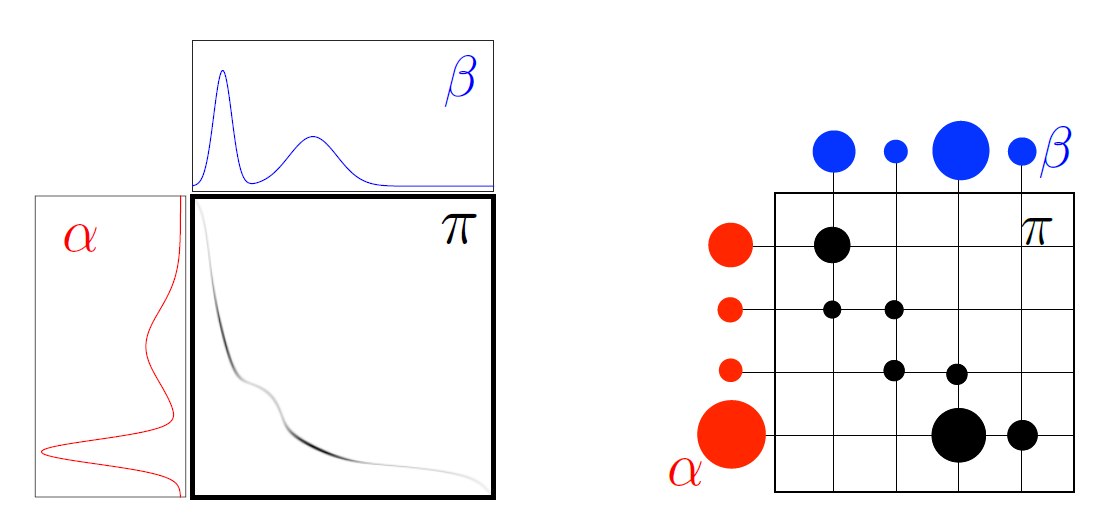
\includegraphics[width=0.7\textwidth]{img/transporte/coupling-example.png}
		  \caption{Izquierda: coupling óptimo entre dos medidas 1-D continuas con densidad. El coupling está localizado a lo largo del grafo del mapa de transporte óptimo $(x, T(x))$. Derecha: coupling óptimo entre dos medidas discretas. El radio del disco negro es proporcional a la masa transportada en esa coordenada. Imagen obtenida de \cite{peyre2019computational}.
			  \label{fig:coupling-example}}
	  \end{figure}


	  En diferencia con el problema de Monge, el problema de Kantorovich siempre tiene solución, si es que $(\cX, \cY)$ son espacios compactos y $c$ es continuo. En efecto, $\Cpl(\mu, \nu)$ es compacto para la topología débil de las medidas, $\pi \mapsto \int c\dd{\pi}$ es una función continua para esta topología, y la restricción $\pi\in\Cpl(\mu, \nu)$ es no vacía. Sigue que existe un coupling óptimo $\pi_{\mu \to \nu}$ que resuelve \eqref{eq:problemaTransporteKantorovich}. Continuando con los ejemplos \ref*{ex:problemaDeMongeSinSolucion} y \ref*{ex:problemaDeMongeMultipleSolucion}, podemos encontrar el coupling óptimo para estos problemas:

	  \begin{example}
		  Sean los espacios $\cX$ y $\cY$ y las medidas $\mu$ y $\nu$ como en el Ejemplo~\ref*{ex:problemaDeMongeSinSolucion}. En este caso, el coupling óptimo entre $\mu$ y $\nu$ corresponde a:
		  \begin{align*}
			  \pi_{\mu \to \nu}\left\{ (-1, 0) \right\} & = \frac{1}{2} & \pi_{\mu \to \nu}\left\{ (1, 0) \right\} & = \frac{1}{2}.
		  \end{align*}
		  Del mismo modo, el coupling óptimo entre $\nu$ y $\mu$ corresponde a:
		  \begin{align*}
			  \pi_{\nu \to \mu}\left\{ (0, -1) \right\} & = \frac{1}{2} & \pi_{\nu \to \mu}\left\{ (0, 1) \right\} & = \frac{1}{2}.
		  \end{align*}

	  \end{example}

	  \begin{example}
		  Del mismo modo, Sean los espacios $\cX$ y $\cY$ y las medidas $\mu$ y $\nu$ como en el Ejemplo~\ref*{ex:problemaDeMongeMultipleSolucion}. En este caso, el coupling óptimo entre $\mu$ y $\nu$ corresponde a:
		  \begin{align*}
			  \pi_{\mu \to \nu}\left\{ ((1, 1), (-1, 1)) \right\}   & = \frac{1}{4} & \pi_{\mu \to \nu}\left\{ ((1, 1), (1, -1)) \right\}   & = \frac{1}{4}  \\
			  \pi_{\mu \to \nu}\left\{ ((-1, -1), (-1, 1)) \right\} & = \frac{1}{4} & \pi_{\mu \to \nu}\left\{ ((-1, -1), (1, -1)) \right\} & = \frac{1}{4}.
		  \end{align*}

	  \end{example}





	  \newpage
	  %   del problema de transporte óptimo, que si tiene solución (aunque puede que no sea única). Este problema se puede definir de la siguiente manera:
	  %   Como se mencionó en la Observación \ref*{remark:problemaTransporteMongeDiscreto}, el problema de transporte óptimo de Monge no siempre tiene solución, y en caso de tenerla, no siempre es única. Motivado por esto, Kantorovich propuso una formulación alternativa del problema de transporte óptimo, que si tiene solución (aunque puede que no sea única). Este problema se puede definir de la siguiente manera:
	  %   \begin{definition}
	  % 	  Dados $\mu \in \ProbSpace[\cX]$ y $\nu \in \ProbSpace[\cY]$, se define el \emph{problema de transporte óptimo de Kantorovich} como el problema de encontrar una medida de probabilidad $\gamma \in \Cpl(\mu, \nu)$ que minimice el costo total de transporte, es decir, que minimice la siguiente expresión:
	  % 	  \begin{equation}
	  % 		  \label{eq:problemaTransporteKantorovich}
	  % 		  \inf_{\gamma \in \Cpl(\mu, \nu)} \int_{\cX \times \cY} c(x, y) \dgamma[x, y] .
	  % 	  \end{equation}
	  % 	  Al conjunto de medidas de probabilidad que resuelven este problema se le llama \emph{transportes óptimos}.\FM[inline]{Se podría agregar el típico dibujo en el que se muestra el copling}
	  %   \end{definition}
	  \FM[inline]{Tenía pensado en poner el teorema de Brenier (teo 2.1 de \cite{peyre2019computational}), pág 27 para explicar la equivalencia Kantorovich-Monge.}


  }

  \section{La Distancia y el Espacio de Wasserstein}\label{sec:la-distancia-y-el-espacio-de-Wasserstein}
  {
	  \FM{Incluir subsections para la distancia, espacio, y convergencia débil?}
	  En esta sección se demostrará que, al evaluar la expresión \eqref{eq:problemaTransporteKantorovich} para una función de coste con distancia, se obtiene una distancia entre medidas de probabilidad. Revisaremos algunas propiedades de esta distancia, para concluir que esta distancia metriza la convergencia débil entre medidas de probabilidad.

	  \begin{definition}[La distancia de Wasserstein]\label{def:distanciaWasserstein}
		  Sea $(\cX, \dist)$ un espacio Polaco y sea $p \geq 1$. Para dos medidas $\mu, \nu$ sobre $\cX$, la distancia de Wasserstein de orden $p$ entre $\mu$ y $\nu$ es definida por medio de la fórmula
		  \begin{equation}
			  \label{eq:distanciaWasserstein}
			  \Wasserstein[p]{\mu}{\nu}  \eqdef \left( \inf_{\gamma \in \Cpl(\mu, \nu)} \int_{\cX \times \cX} \dist(x, y)^{p} \dgamma[x, y] \right)^{\frac{1}{p}}.
		  \end{equation}

	  \end{definition}

	  \begin{example}
		  $\Wasserstein[1]{\delta_x}{\delta_y} = \dist(x, y)$. Notemos que en este ejemplo, se puede interpretar que la distancia de Wasserstein metriza el ``esfuerzo'' de llevar la masa del punto $x$ al punto $y$.
	  \end{example}

	  Notemos que, en estricto rigor, $W_p$ no es una distancia en sí, dado que puede tomar valores de $+\infty$, sin embargo, se puede demostrar que $W_p$ satisface los axiomas de ser una distancia. No se demostrará este hecho, pero se puede encontrar una demostración en \cite{villani2009optimal}, pág 94.

	  Por tanto, resulta natural definir el espacio en el que la distancia de Wasserstein tome valores finitos.

	  \begin{definition}[El espacio de Wasserstein]
		  Con los mismos supuestos que en la Definición \ref{def:distanciaWasserstein}, se define el espacio de Wasserstein de orden $p$ por medio de
		  \begin{equation}
			  \WassersteinSpace[p]{\cX} \eqdef \left\{
			  \mu \in \ProbSpace[\cX] \colon \int_{\cX} \dist(x, x_0)^{p} \dmu[x] < \infty
			  \right\},
		  \end{equation}
		  donde $x_0 \in \cX$ es un punto fijo arbitrario. De esta forma, $W_p$ define una distancia (finita) sobre $\WassersteinSpace[p]{\cX}$.
	  \end{definition}
	  En palabras simples, el espacio de Wasserstein de orden $p$ es el conjunto de medidas de probabilidad en $\cX$ cuyo momento de orden $p$ es finito. Lo interesante del espacio de Wasserstein, es que su respectiva distancia lo metriza, como lo dice el siguiente teorema:
	  \begin{theorem}\label{thm:espacioWassersteinEsMetrico}
		  Si $(\cX, \dist)$ es un espacio Polaco, entonces el espacio de Wasserstein $\WassersteinSpace[p]{\cX} $, metrizado por la distancia de Wasserstein $W_p$, es también un espacio Polaco.
	  \end{theorem}

	  \begin{proof}
		  Revisar la demostración del Teorema 6.18 en \cite[p. 105]{villani2009optimal}
	  \end{proof}

	  A partir de ahora, se asumirá que el espacio $\WassersteinSpace[p]{\cX} $ siempre estará equipado con su respectiva distancia $W_p$.

	  \begin{remark}
		  A través de la desigualdad de Hölder, se puede demostrar que para $p \leq q$, se tiene que $\Wasserstein[p]{\mu}{\nu} \leq \Wasserstein[q]{\mu}{\nu}$, para toda $\mu, \nu \in \WassersteinSpace[p]{\cX}$. Y por tanto, las topologías inducidas por las distancias de Wasserstein se van encajonando.

		  En particular, la distancia de Wasserstein de orden 1, es la más débil de todas. Como norma general, la distancia $W_1$  es la más flexible y fácil de acotar, mientras que la distancia $W_2$ posee mejores propiedades geométricas, pero es más difícil de trabajar.
	  \end{remark}

	  Vista la distancia y el espacio de Wasserstein, se presentará una caracterización de convergencia en este espacio. Para ello, se definirá la convergencia débil entre medidas de probabilidad.

	  \begin{definition}[Convergencia Débil]
		  Sea $(\cX, \dist)$ un espacio Polaco y sea $p \geq 1$. Se dice que una sucesión de medidas de probabilidad $(\mu_n)_{n \in \N} \subset \WassersteinSpace[p]{\cX} $ converge débilmente a $\mu \in \WassersteinSpace[p]{\cX}$ si
		  \begin{equation}
			  \forall \phi \in \ContBoundedSpace[\cX], \quad \int_{\cX} \phi(x) \dd{\mu_n(x)} \to \int_{\cX} \phi(x) \dmu[x].
		  \end{equation}
		  y lo denotaremos por $\mu_n \wto \mu$.
	  \end{definition}

	  \begin{note}
		  Intuitivamente, que una sucesión de medidas de probabilidad converjan débilmente a una medida $\mu$ significa que es la forma ``más fácil'' que tiene la sucesión de converger a $\mu$.
	  \end{note}

	  \begin{theorem}[La Distancia de Wasserstein Metriza la Convergencia Débil]
		  Sea $(\cX, \dist)$ un espacio Polaco y sea $p \geq 1$. Entonces, la distancia de Wasserstein $W_p$  metriza la convergencia débil en $\WassersteinSpace[p]{\cX}$.
	  \end{theorem}

	  \begin{remark}
		  En otras palabras, si $(\mu_n)_{n\in\N}$ es una sucesión de medidas de probabilidad en $\WassersteinSpace[p]{\cX}$ y $\mu\in \WassersteinSpace[p]{\cX} $ otra medida, entonces $\mu_n \wto \mu$ si y sólo si $\Wasserstein[p]{\mu_n}{\mu} \to 0$.
	  \end{remark}

	  \begin{example}
		  Consideremos las siguientes distancias y divergencias entre medidas de probabilidad:
		  \begin{gather*}
			  \TV{\mu}{\nu} \eqdef \sup_{A \subseteq \cX} \abs{\mu(A) - \nu(A)}, \\
			  \KL{\mu}{\nu} \eqdef \int_{\cX} \log\left(\dv{\mu}{\nu}(x)\right) \dmu[x], \\
			  \JS{\mu}{\nu} \eqdef \KL{\mu}{\frac{\mu + \nu}{2}} + \KL{\nu}{\frac{\mu + \nu}{2}},
		  \end{gather*}
		  donde la primera es la distancia total variación, la segunda es la divergencia de Kullback-Leibler, y la tercera es la divergencia de Jensen-Shannon.

		  Si consideramos $\delta_\theta$ y $\delta_0$ medidas de Dirac centradas en $\theta$ y $0$ respectivamente, entonces se puede demostrar que
		  \begin{align*}
			  \Wasserstein[1]{\delta_\theta}{\delta_0} & = |\theta|                            &
			  \TV{\delta_\theta}{\delta_0}             & = \begin{cases}
				                                               1 & \text{si } \theta \neq 0 \\
				                                               0 & \text{si } \theta = 0
			                                               \end{cases}          \\
			  \KL{\delta_\theta}{\delta_0}             & = \begin{cases}
				                                               +\infty & \text{si } \theta \neq 0 \\
				                                               0       & \text{si } \theta = 0
			                                               \end{cases} &
			  \JS{\delta_\theta}{\delta_0}             & = \begin{cases}
				                                               \log(2) & \text{si } \theta \neq 0 \\
				                                               0       & \text{si } \theta = 0
			                                               \end{cases}
		  \end{align*}
		  Entonces, si tomamos $\theta = \frac{1}{n} $ y dejamos que $n \to \infty$, se tiene que $\Wasserstein[1]{\delta_\theta}{\delta_0} \to 0$, pero el resto de distancias y divergencias no convergen a 0.
		  Por tanto, se puede notar que la distancia de Wasserstein es la única que es capaz de distinguir entre medidas de probabilidad que no tienen soporte en el mismo punto, gracias a que metriza la convergencia débil.
	  \end{example}

  }  % end of sec. La Distancia y el Espacio de Wasserstein

  \section{El Baricentro de Wasserstein Bayesiano}\label{sec:el-baricentro-de-Wasserstein-Bayesiano}
  {
	  \subsection*{La Media de Fréchet}\label{ssec:la-media-de-Frechet}
	  {
		  En esta sección se revisará el concepto de media de Fréchet, el cual es una generalización de la noción de promedio para espacios métricos. Este concepto será clave para definir el baricentro de Wasserstein.
		  \begin{definition}[Funcional y Media de Fréchet]
			  Sea $(\cX, \dist)$ un espacio Polaco. Sean $x_1,$ $\ldots, x_n$ puntos en $\cX$ y sean $w_1,\ldots,w_n\in\R$ pesos asociados a los puntos. Para cada $p\in\cX$, se define el \emph{funcional de Fréchet} por
			  \begin{equation}
				  \label{eq:funcionalFrechet}
				  \Psi(p) \eqdef \sum_{i=1}^{n} w_i \dist(p, x_i)^2.
			  \end{equation}
			  Y, en caso de que exista un punto $m \in \cX$ que minimice el funcional $\Psi$, entonces este se definirá como la \emph{media de Fréchet} de los puntos $x_1,\ldots, x_n$. Es decir, es aquel punto tal que minimiza el siguiente problema:
			  \begin{equation}
				  \label{eq:mediaFrechet}
				  m \eqdef \argmin_{p \in \cX} \sum_{i=0}^{n} w_i \dist(p, x_i)^2.
			  \end{equation}
		  \end{definition}

		  \begin{example}\label{ex:baricentro-triangulo}
			  Tomemos $x_1, x_2, x_3 \in \R^2$ tres puntos en el plano, formando un triángulo. Si se define el promedio (o el \textit{baricentro}, en el contexto de un triángulo) de estos puntos por $\bar x = \frac{1}{3} (x_1 + x_2 + x_3)$, entonces se puede comprobar fácilmente que este es el único que minimiza el funcional de Fréchet:
			  \begin{equation}
				  F(p) = \frac{1}{3} \sum_{i=0}^{3} \|p - x_i\|^2.
			  \end{equation}
			  Dado que este funcional se puede descomponer de la siguiente manera:
			  \begin{equation}
				  F(p) = F(\bar x) + \|p-\bar x\|^2,
			  \end{equation}
			  se puede ver que la media de Fréchet generaliza la noción de promedio.
		  \end{example}

		  \begin{remark}
			  La razón por la que resulta interesante estudiar este concepto, es que sólo utiliza nociones métricas, y se desliga de la noción vectorial. Como se vió en el Ejemplo \ref{ex:baricentro-triangulo}, el promedio utilizó nociones vectoriales (suma, ponderación) mientras que la media de Fréchet utilizó nociones métricas, resultando en el mismo promedio.

			  Sin embargo, el hecho de que se pueda cambiar la distancia, hace que el baricentro cambie, y dependa de ésta.
		  \end{remark}



	  }  % end of sec. La Media de Fréchet

	  \subsection*{El Baricentro de Wasserstein}\label{ssec:el-baricentro-de-Wasserstein}
	  {
		  Como se vió en la sección anterior, la media de Fréchet permite definir una noción de promedio, en espacios métricos. El Teorema \ref{thm:espacioWassersteinEsMetrico} nos dice que $(\WassersteinSpace[p]{\cX}, W_p)$ es un espacio métrico, y por tanto, se puede definir su respectivo ``promedio'':
		  \begin{definition}
			  Sean $\mu_1,\ldots, \mu_n \in \WassersteinSpace[p]{\cX} $ y sean $w = (w_1,\ldots, w_n) \in \Simplex[n]$ sus pesos asociados. El \emph{baricentro de Wasserstein} se define por medio de
			  \begin{equation}
				  \bar \mu \eqdef \arginf_{\nu \in \WassersteinSpace[p]{\cX} } \sum_{i=0}^{n} w_i \Wasserstein[p]{\nu}{\mu_i}^p
			  \end{equation}

		  \end{definition}
		  \FM[inline]{Se podría poner algún ejemplo con una imagen.}

		  Es posible generalizar aún más la noción de baricentro de Wasserstein a una colección infinita de medidas. Esto se puede hacer considerando una medida $\Gamma \in \ProbSpace[\ProbSpace ] $, que cumplirá el rol de los pesos $w_1,\ldots, w_n $ en la definición anterior. Esto se puede formalizar en la siguiente definición:

		  \begin{definition}
			  Sea $\Gamma \in \ProbSpace[\ProbSpace]$ una medida. El baricentro de Wasserstein se puede (re)-definir como aquel que minimice el siguiente problema:
			  \begin{equation}
				  \bar \mu \eqdef \arginf_{\mu \in \ProbSpace} \int_{\ProbSpace} \Wasserstein[p]{\mu}{\nu}^p \dd{\Gamma(\nu)}
			  \end{equation}

		  \end{definition}


	  }  % end of sec. El Baricentro de Wasserstein


	  \subsection{Geodésicas en el Espacio de Wasserstein}\label{ssec:geodesicas-Wasserstein}
	  {
		  En esta sección, se utilizará la distancia de Wasserstein para definir una noción de geodésica en el espacio de Wasserstein. Esta noción será de utilidad para definir el baricentro de Wasserstein Bayesiano.
		  \FM[inline]{Agregar la referencia del Lecture}
		  \begin{definition}
			  Sea $(\cX, \dist)$ un espacio métrico. Una \emph{geodésica a velocidad constante}  entre dos puntos, $x_0, x_1 \in \cX$ es una curva continua $x : [0, 1] \to \cX$  tal que para cada $s, t \in [0, 1]$, $\dist(x_s,x_t) = |s - t| \dist(x_0,x_1) $.
		  \end{definition}

		  \begin{proposition}
			  Sean $\mu_0, \mu_1 \in \WassersteinSpace[p]{\cX} $, con $\cX \in \R^d$  compacto y convexo. Sea $\gamma \in \Cpl(\mu_0, \mu_1)$  un plan de transporte óptimo\FM{Agregar en la def que estos se llamarán planes de transporte}. Definamos
			  \begin{equation}
				  \mu_t \eqdef \pf{(\pi_t)} \gamma, \quad \text{donde } \pi_t(x, y) = (1-t)x + ty.
			  \end{equation}
			  Entonces, la curva $\mu_t$ es una geodésica a velocidad constante entre $\mu_0$ y $\mu_1$.

		  \end{proposition}

		  \begin{example}
			  Si existe un mapa de transporte óptimo $T$ entre $\mu_0$ y $\mu_1$, entonces la geodésica definida arriba es $\mu_t = \pf{((1-t)\id + tT)} \mu_0$.
		  \end{example}

		  \begin{remark}
			  En caso en que $\mu_0 = \sum_{i=1}^{n} m_i \delta_{x_i}$ y $\mu_1 = \sum_{i=1}^{n} m_i \delta_{y_i}$, con $m\in\Simplex[n]$ y $x_1,\ldots, x_n, y_1,\ldots, y_n \in \cX$, entonces la geodésica definida arriba se puede escribir de la siguiente manera:
			  \begin{equation}
				  \mu_t = \sum_{i=1}^{n} m_i \delta_{(1-t)x_i + ty_i},
			  \end{equation}
			  lo que se puede interpretar como que la masa $m_i$ del punto $x_i$ se transporta al punto $y_i$ a velocidad constante.
		  \end{remark}




	  }  % end of sec. Geodésicas en el Espacio de Wasserstein

	  \subsection{El Baricentro de Wasserstein Bayesiano}\label{ssec:baricentro-Wasserstein-Bayesiano}
	  {
		  \FM[inline]{Comentar que aquí se está tomando ideas de la tesis de Gonzalo Ríos}
		  Consideremos muestras $\Data = \left\{ x_1,\ldots, x_n  \right\}$ en un espacio $\cX$ y un conjunto de modelos factibles o medidas de probabilidad $\Models \subseteq \ProbSpace[\cX]$. Aprender un modelo, también conocido como la \emph{selección de un modelo}, de $\Data$ consiste en escoger un elemento $\mu \in \Models$ que mejor explique los datos, si es que estos hubieran sido generados por $\mu$, dado algún criterio.

		  Se considerará una medida de probabilidad $\Prior \in \ProbSpace[\Models]$ sobre un espacio de modelos $\Models$  un \emph{prior} fijo.
	  }  % end of sec. El Baricentro de Wasserstein Bayesiano

  }  % end of sec. El Baricentro de Wasserstein

 }